\begin{framed}

Objetivos:
\begin{itemize}
    \item Introducir la función corriente.
    \item Estudiar el flujo irrotacional. 
    \item Presentar la función potencial.
\end{itemize}

Contenidos:
\begin{itemize}
    \item Flujo incompresible y la función corriente.
    \begin{itemize}
        \item Definición e implicancias físicas
        \item Formulación alternativa de Navier Stokes con la función corriente
    \end{itemize}
    \item La circulación y su relación con la vorticidad.
    \item Flujo irrotacional y la función potencial.
\end{itemize}

Bibliografía:
\begin{itemize}
    \item White, F. M. (2008) Mecánica de Fluidos. McGraw-Hill. Sexta edición. Secciones 4.7-4.9
    \item Fox, R. W., Pritchard, P. J. y McDonald, A. T. (2009) Introduction to Fluid Mechanics. John Wiley \& Sons. Secciones 5.2, 5.3, 6.7.
\end{itemize}
\end{framed}

\section*{La función corriente}

La clase pasada revisamos la ley de conservación de masa, que deriva en la ecuación de continuidad:
%
\begin{equation} \label{eq:continuidad_2}
\frac{\partial \rho}{\partial t} + \frac{\partial(\rho u)}{\partial x} + \frac{\partial(\rho v)}{\partial y} + \frac{\partial(\rho w)}{\partial z} = 0.
\end{equation}
%
En el caso particular de dos dimensiones e incompresible, la Ec. \eqref{eq:continuidad_2} se reduce a
%
\begin{equation} \label{eq:continuidad2D}
\frac{\partial u}{\partial x} + \frac{\partial v}{\partial y} = 0.
\end{equation}

La ecuación \eqref{eq:continuidad2D} sería satisfecha automáticamente si existiese una función $\psi$ tal que
%
\begin{equation} \label{eq:psi_def}
u = \frac{\partial \psi}{\partial y} \quad v = -\frac{\partial \psi}{\partial x}.
\end{equation}
%
De hecho, si reemplazamos la Ec. \eqref{eq:psi_def} en la Ec. \eqref{eq:continuidad2D}, claramente el lado izquierdo de la Ec. \eqref{eq:continuidad2D} se hace cero.

\subsection*{Interpretación geométrica de $\psi$}
El truco de usar una función $\psi$ va más allá de lo puramente matemático, ya que tiene una interpretación geométrica: la líneas de $\psi$ constante son líneas de flujo.
Esto significa que si seguimos una partícula que va con el fluido, su trayectoria estaría definida por una línea de $\psi =\text{constante}$.
Por esta razón, conocemos a $\psi$ como la \emph{función corriente}.

\begin{figure}[!h]
\centering
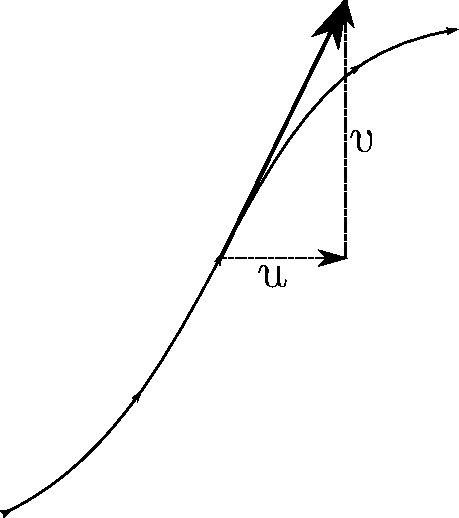
\includegraphics[width=0.3\textwidth]{clase02/flujo.pdf}
\caption{Línea de flujo bidimensional.}
\label{fig:flujo}
\end{figure}

Demostremos esta propiedad de $\psi$.
Como lo muestra la Figura \ref{fig:flujo}, la velocidad es siempre tangencial a una línea de flujo. 
En otras palabras, la trayectoria debe tener la misma pendiente que la velocidad, o
%
\begin{align}\label{eq:linea_flujo}
\frac{dy}{dx} = \frac{v}{u} \nonumber \\
\Rightarrow udy - vdx = 0.
\end{align}
%
La segunda expresión de la Ec. \eqref{eq:linea_flujo} determina una línea de flujo, y reemplazando la definición de $\psi$ de la Ec. \eqref{eq:psi_def} llegamos a
%
\begin{equation}
\frac{\partial\psi}{\partial x} dx + \frac{\partial \psi}{\partial y}dy = 0 = d\psi,
\end{equation}
%
lo cual es la definición de derivada total.
Si $d\psi=0$, $\psi$ debe ser constante a lo largo de una línea de flujo.

Esta propiedad de $\psi$ es muy útil para visualizar flujos.
De hecho, en visualizaciones de modelación computacional de fluidos, comúnmente es la funcion corriente la que se grafica.

\subsection*{Interpretación física de $\psi$}

\begin{figure}[!h]
\centering
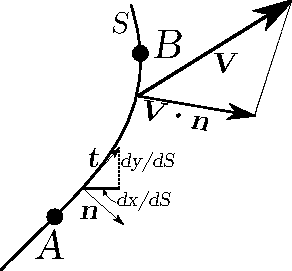
\includegraphics[width=0.5\textwidth]{clase02/caudal.pdf}
\caption{Caudal entre los puntos $A$ y $B$.}
\label{fig:caudal}
\end{figure}

La función corriente también es útil para calcular el caudal que pasa por una superficie.
Usemos la Figura \ref{fig:caudal} para guiar esta explicación.
Digamos que $S$ es una superficie que pasa por los puntos $A$ y $B$ (acuérdense que estamos trabajando en dos dimensiones, por lo que una superficie corresponde a una línea), y queremos saber el caudal que pasa por $S$ entre $A$ y $B$.
Por definición, el caudal a través de un diferencia de $S$ ($dS$) es 
%
\begin{equation}\label{eq:caudal}
dQ = \mathbf{V}\cdot\mathbf{n}dS,
\end{equation}
%
donde $\mathbf{n}$ es un vector unitario normal a la superficie, y $\mathbf{V}=u\ihat+v\jhat=u = \frac{\partial \psi}{\partial y} \ihat -\frac{\partial \psi}{\partial x}\jhat$.

\mbox{?`}Cómo podemos encontrar una expresión para $\mathbf{n}$? Debemos recurrir a nuestros conocimientos de algebra lineal.
Si la función que define $S$ es $y=y(x)$, $dx\ihat+dy\jhat$ es un vector tangencial a $S$.
Así, podemos calcular el vector tangencial unitario, que es $\mathbf{t}=(dx\ihat+dy\jhat)/\sqrt{dx^2+dy^2}$, donde $\sqrt{dx^2+dy^2}=dS$ es el tamaño del elemento diferencial de la curva $S$.
Sabemos que el producto punto entre $\mathbf{t}$ y $\mathbf{n}$ debe ser cero, por lo tanto, el vector normal a $S$ tiene la forma
%
\begin{equation}\label{eq:vec_normal}
\mathbf{n} = \frac{dy}{dS}\ihat - \frac{dx}{dS}\jhat.
\end{equation}
%
Si insertamos la Ec. \eqref{eq:vec_normal} en la Ec. \eqref{eq:caudal}, quedamos con:
%
\begin{align}
dQ &= \left(\frac{\partial \psi}{\partial y} \ihat -\frac{\partial \psi}{\partial x}\jhat\right)\cdot\left( \frac{dy}{dS}\ihat - \frac{dx}{dS}\jhat\right)dS\nonumber\\
   &= \frac{\partial \psi}{\partial y}dy +\frac{\partial \psi}{\partial x}dx = d\psi
\end{align}
%
Por lo tanto, el caudal total que pasa por $S$ entre $A$ y $B$ es
\begin{equation}\label{eq:caudal_psi}
Q=\int_A^BdQ = \int_A^Bd\psi = \psi_B-\psi_A.
\end{equation}
%
En otras palabras, el caudal entre $A$ y $B$ es solamente la diferencia entre la función corriente evaluada en esos dos puntos, sin importar la forma de la superficie $S$ entre ellos.

\paragraph*{Ejemplo}
(Sacado de \emph{Fluid Mechanics}, Munson et al.)
Un flujo incompresible bidimensional tiene velocidad $\mathbf{V}=u\ihat+v\jhat$, con $u=2x$
{\bf (a)}Calcule $v$ sabiendo que es cero sobre el eje $x$.
{\bf (b)}Encuentre la velocidad promedio del fluido cruzando una superficie recta que une el centro del eje coordenado con el punto $(1,1)$.

Al ser incompresible, sabemos que:
%
\begin{align}
&\frac{\partial u}{\partial x} + \frac{\partial v}{\partial y} = 0 \nonumber \\
\Rightarrow &\frac{\partial v}{\partial y} = -\frac{\partial u}{\partial x} = -2 \nonumber \\
\Rightarrow &v = -2y + C_1(x),
\end{align}
%
donde $C_1(x)$ es una función de $x$.
Nos dicen que la $v=0$ sobre el eje $x$ (donde $y=0$), por lo que $C_1(x)=0$.

Podemos encontrar la velocidad promedio dividiendo el caudal por el área, y para calcular el caudal necesitamos $\psi$.
Viendo la definición de $\psi$ en la Ec. \eqref{eq:psi_def}, podemos decir que
%
\begin{equation}
\psi = \int u dy = 2xy + C_2(x)
\end{equation}
%
e insertando ese resultado en la segunda expresión de la Ec. \eqref{eq:psi_def}, llegamos a
%
\begin{equation}
v = -\frac{\partial \psi}{\partial x} = -2y - \frac{dC_2}{dx}.
\end{equation}
%
Antes calculamos que $v=-2y$, por lo tanto, $dC_2/dx=0$ y $C_2$ es una constante
\mbox{?`}Qué constante? En verdad, da lo mismo, y la podemos dejar en $C_2=0$, pero cualquier constante cumple con los requerimientos.
Nosotros estamos preocupados de variaciones de $\psi$ más que $\psi$ en si, así que el valor de la constante es irrelevante.

La Ec. \eqref{eq:caudal_psi} nos dice que el caudal a través de cualquier superficie que pase por los puntos $(0,0)$ y $(1,1)$ es la diferencia de $\psi$ evaluada en esos puntos, lo que es $Q=2-0=2$.
Nos especificaron que la superficie es una línea recta entre esos puntos, por lo que el área no es más que la distancia entre ellos: $d=\sqrt{2}$, y la velocidad promedio $Q/d=1$.

\subsection*{Relación de $\psi$ con la vorticidad y la ecuación de Navier-Stokes.}

Vimos la clase pasada que la vorticidad es $\nabla \times\mathbf{V}$, lo que en dos dimensiones es
%
\begin{equation}\label{eq:vort_2D}
\boldsymbol{\omega}=\left(\frac{\partial v}{\partial x}-\frac{\partial u}{\partial y} \right) \khat.
\end{equation}
%
El reemplazo $\psi$ de la Ec. \eqref{eq:psi_def} en la Ec. \eqref{eq:vort_2D}, nos entrega
%
\begin{equation}\label{eq:vort_laplace}
\boldsymbol{\omega}=\left[\frac{\partial}{\partial x}\left(-\frac{\partial \psi}{\partial x}\right) -\frac{\partial}{\partial y}\left(\frac{\partial \psi}{\partial y}\right) \right] = -\nabla^2\psi\khat
\end{equation}
%
lo que relaciona $\psi$ con $\boldsymbol{\omega}$.

A partir de esto, podemos obtener una formulación diferente de la ecuación de Navier-Stokes, en función de $\psi$ (y/o $\boldsymbol{\omega}$).
Para que se acuerden, Navier-Stokes en forma vectorial es:
%
\begin{equation}\label{eq:NS_2}
\frac{D\mathbf{V}}{Dt} = -\frac{\nabla p}{\rho} + \nu\nabla^2\mathbf{V}.
\end{equation}
%
Si le sacamos el rotor a la Ec. \eqref{eq:NS_2} obtenemos
%
\begin{align}\label{eq:transp_vort}
\frac{D(\nabla\times\mathbf{V})}{Dt} &= \underbrace{-\frac{\nabla\times\nabla p}{\rho}}_{=0} + \nu\nabla^2(\nabla\times\mathbf{V}). \nonumber\\
\frac{D \omega_z}{Dt} &= \nabla^2 \omega_z,
\end{align}
%
donde $\nabla\times\nabla p=0$ pues el rotor de un gradiente es siempre cero (revisen sus cuadernos de matemáticas, o pruebenlo!) .

La Ec. \eqref{eq:transp_vort} se conoce como la ecuación de transporte de vorticidad, en donde la vorticidad es ``transportada'' por el flujo, tal como si fuera la concentración de algún contaminante.
El caso tridimensional es más complicado pues aparece un término extra conocido como ``estiramiento de vorticidad'', el cual tiene profundas implicancias en la teoría de turbulencia.
Usando la Ec. \eqref{eq:vort_laplace}, llegamos a la formulación de Navier-Stokes con la función corriente
%
\begin{equation}\label{eq:NS_psi}
\frac{D(\nabla^2\psi)}{Dt} = \nu\nabla^4\psi.
\end{equation}

Usar la Navier-Stokes en las formas de las Ecs. \eqref{eq:transp_vort} o \eqref{eq:NS_psi} tiene la gran ventaja que no hay que preocuparse de la presión, y que la incompresibilidad se satisface automáticamente. 
El problema es que las condiciones de borde se enfuerzan naturalmente en la velocidad (impermeabilidad $\mathbf{V}\cdot\mathbf{n}=0$ y no deslizamiento $\mathbf{V}=0$), y necesitamos derivar su símil para $\psi$ o $\omega_z$ (y para el caso de $\psi$ necesitamos cuatro condiciones de contorno!).

\section*{La vorticidad}
La clase anterior definimos la vorticidad como el rotor de la velocidad:
%
\begin{equation}\label{eq:vort_2}
\boldsymbol{\omega} = \nabla\times\mathbf{V},
\end{equation}
%
que (como sabrán ustedes), resulta en un vector.
Vimos también que la vorticidad está relacionada con la rotación y deformación angular de un elemento de fluido: si $\boldsymbol{\omega}=0$, el elemento de fluido no está rotando ni deformándose angularmente.
No se confundan: que $\boldsymbol{\omega}=0$ no significa que el elemento de fluido no pueda tener una trayectoria curva, como lo muestra la Figura \ref{fig:irrotacional}.
%
\begin{figure}[!h]
\centering
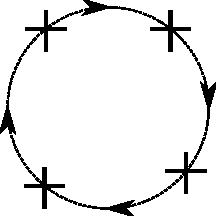
\includegraphics[width=0.3\textwidth]{clase02/irrotacional.pdf}
\caption{Flujo irrotacional con trayectoria curva.}
\label{fig:irrotacional}
\end{figure}
%
Intuitivamente, uno diría que $\boldsymbol{\omega}\neq 0$ en el flujo de la Figura \ref{fig:irrotacional}, sin embargo, fíjense en la cruz, que mantiene su aspecto todo el tiempo. 
La velocidad va cayendo a medida que nos alejamos del centro de tal manera que la cruz no rota ni pierde su forma, por lo tanto, la vorticidad del flujo es $0$.
A este tipo de flujo se les llama \emph{irrotacionales}.

\paragraph*{Implicancia física del flujo irrotacional.}
Si un flujo es irrotacional, el elemento de fluido no rota ni se deforma angularmente. 
Por lo tanto los esfuerzos de corte en la superficie del elemento de fluido ($\tau_{ij}$ en la clase pasada) deben ser cero.

Por otra parte, en un fluido Newtoniano, el esfuerzo de corte y la velocidad se relacionan a través de la viscosidad $\mu$.
Esto significa que un fluido sin viscosidad no es capaz de generar esfuerzos de corte $\tau_{ij}$, y por ende, de generar un rotacional.
Así llegamos a una implicancia física: si un flujo no viscoso inicialmente tiene rotor $\nabla\times\mathbf{V}=0$, la vorticidad será siempre $\boldsymbol{\omega}=0$.

\paragraph*{Implicancia matemática del flujo irrotacional.}
Se acordarán de sus cursos de matemáticas de que un campo vectorial con rotor cero puede ser representado como la gradiente de un campo escalar.
Este es exactamente el caso cuando un flujo es irrotacional: la velocidad es un campo vectorial con rotor cero, por lo tanto debe haber una función ($\phi$) tal que $\mathbf{V} = \nabla\phi = \frac{\partial \phi}{\partial x}\ihat + \frac{\partial \phi}{\partial y}\jhat$

\paragraph*{Vorticidad y circulación}
Nuevamente, se acrodarán de sus cursos de matemáticas del concepto de circulación ($\Gamma$).
Ésta es la integral cerrada de un campo vectorial (en este caso, la velocidad) a lo largo de una curva:
%
\begin{equation}\label{eq:circulacion}
\Gamma = \oint_L \mathbf{V}\cdot\mathbf{t}dl,
\end{equation}
%
donde $\mathbf{t}$ es un vector unitario tangente a la curva $L$, y $dl$ es un elemento diferencial de $L$.
La circulación es una cantidad que cuesta interpretar físicamente, pero podemos operar sobre la ecuación \eqref{eq:circulacion} para visualizarlo más claramente.
El teorema de Stokes (de nuevo, revisen sus cuadernos de matemáticas, o Google), nos permite pasar de una integral de línea a una de área:
%
\begin{equation}
\oint_L\mathbf{V}\cdot\mathbf{t}dl = \int\int_A\nabla\times\mathbf{V}dS,
\end{equation}
%
donde $A$ es el área encerrada por la curva $L$ y $dS$ es un elemento diferencial de $A$.
Fácilmente pueden reconocer el integrando dentro de la integral de área como la vorticidad. 
En dos dimensiones llegamos a
%
\begin{equation}\label{eq:circ_vort}
\Gamma = \oint_L\mathbf{V}\cdot\mathbf{t}dl = \int\int_A\omega_zdS
\end{equation}

La Ec. \eqref{eq:circ_vort} nos entrega más información del significado físico de la circulación: es la rotación y deformación angular de una región del fluido ($A$), y la vorticidad no es más que la circulación por unidad de área.
De hecho, en el caso de un fluido no viscoso ($\nu=0$), podemos reescribir la Ec. \eqref{eq:transp_vort} como $D\boldsymbol{\omega}/Dt=0$, lo que implica que
%
\begin{equation}\label{eq:teorema_kelvin}
\frac{D\Gamma}{Dt}=0,
\end{equation}
%
lo que se conoce como el \emph{teorema de circulación de Kelvin}.
\mbox{?`}Qué significa este teorema físicamente? Ustedes saben que $D()/Dt$ es la variación en el tiempo de una cantidad que se mueve con el fluido; pues la circulación de una región del fluido (que se mueve con este) se mantiene constante si no hay fuerzas viscosas ($\tau$).
Más simple, si hay una colección de moléculas que estan girando y/o deformándose angularmente, lo van a seguir haciendo al mismo ritmo si no hay viscosidad.  

\section*{Flujo potencial}
Detengámonos en la implicancia matemática del flujo irrotacional.
Dijimos que al tener rotor nulo, existe una función escalar $\phi$ tal que $\mathbf{V}=\nabla\phi$, y $\phi$ se conoce como la función potencial.
Si a esto le agregamos la suposición de flujo incompresible ($\nabla\cdot\mathbf{V}=0$), llegamos a
%
\begin{equation}\label{eq:laplace_phi}
\nabla\cdot\mathbf{V} = \nabla\cdot\nabla\phi = \nabla^2\phi=0.
\end{equation}

La Ec. \eqref{eq:laplace_phi} es una ecuación de Laplace, y los flujos que se pueden representar de esta manera se conocen como \emph{flujo potencial}.

Recapitulemos para evitar confusión:
\begin{itemize}
\item Si un flujo es incompresible y bidimensional, hay una función corriente $\psi$ que describe las líneas de flujo cuando $\psi=$constante.
\item Si un flujo es irrotacional, existe una función potencial $\phi$ (escalar) tal que su gradiente es igual a la velocidad $\nabla\phi=\mathbf{V}$.
\item Si un flujo es ideal (incompresible y no viscoso), es un flujo potencial y se cumple la ecuación de Laplace $\nabla^2\phi=0$.
\end{itemize}
